\newpage
\section{Grundlagen IT und IM} \label{infos}
Siehe auch Wissenschaftliches Arbeiten~\footcite[\vglf][S. 1]{Balzert.2008}. %ohne textcommands
Damit sollten alle wichtigen Informationen abgedeckt sein ;-)~\footcite[\vglf][\pagef 1]{Balzert.2008} %mit textcommands
Hier gibt es noch ein Beispiel für ein direktes Zitat\footcite[][\pagef 1]{Balzert.2008} %mit textcommands

\subsection{Wissenspyramide}

Information = Angabe von Sachverhalten und Vorgängen; zweckbezogen
\\Wissen = Information, die aufgrund von Erfahrung oder durch logische Ableitung begründet ist.

\begin{figure}[H]
\caption{Wissenspyramide}
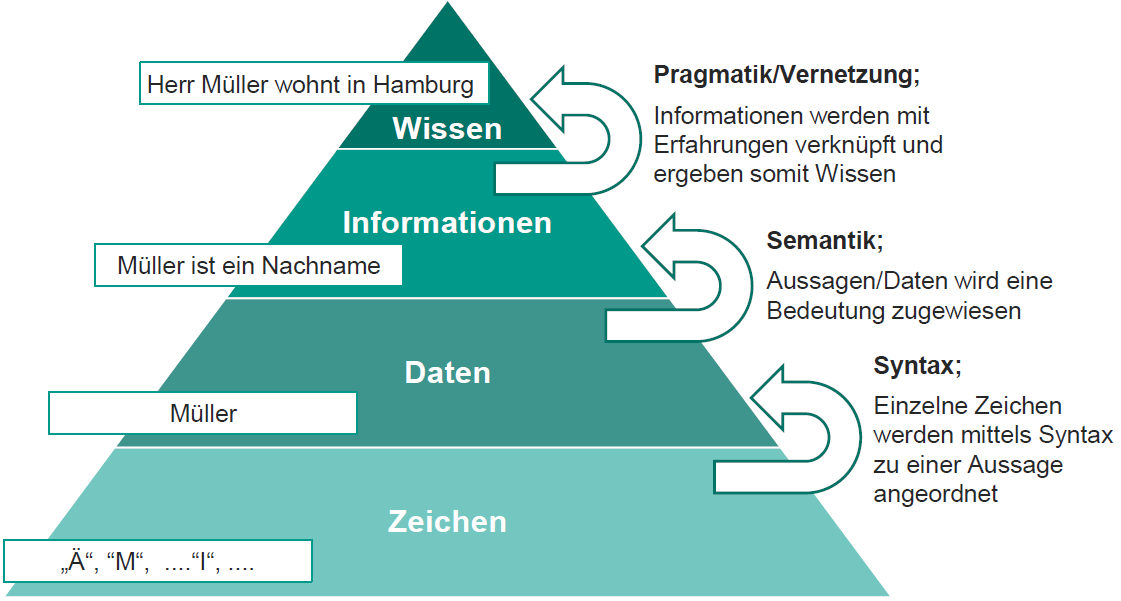
\includegraphics[width=0.9\textwidth]{wissenspyramide}
\\
\cite[Quelle: Vgl.][]{FOM}
\end{figure}
Management beinhaltet
\\Analysen, Entscheidungen, Bewertungen, Kontrollen (Ansoff)
\\umfasst (nach Malik) Setzen von Zielen und Visionen, Organisieren, Entscheiden, Kontrollieren, Menschen zu entwickeln und zu fördern

Informationsmanagement
\begin{itemize}
\item zentrale Führungsaufgaben im Unternehmen
\begin{itemize}
    \item Informationswirtschaft (Angebot, Nachfrage, Verwendung von Informationen)
    \item Informationssysteme (Daten, Prozesse, Anwendungslebenszyklus)
    \item IuK-Technologie (Speicherung, Verarbeitung, Kommunikation)
\end{itemize}

\item unterstützen die wertschöpfenden Prozesse
\end{itemize}

Informations- und Kommunikationstechnik
\begin{itemize}
    \item ist Quartärer Wirtschaftssektor, verbunden mit primärem (Urproduktion, Rohsoffen), sekundärem (Herstellung und Verarbeitung) und tertiären Wirtschaftssektor (Dienstleistungen, Banken)
    \item Verschiedene Entwicklungsstufen
    \begin{itemize}
        \item Unterstützung der Organisationssstrategie (ganzheitl. Sicht)
        \item Unterstützung der Wettbewerbsstrategie (Automat. Wettbewerbs- und Marktbeobachtung)
        \item Unterstützung des Managements
        \item Unterstützung operativer Abläufe
    \end{itemize}
\end{itemize}

\textbf{Wissensmanagement} \\
\\Warum unterstützen?
\begin{itemize}
    \item Wissen ist "flüchtig"
    \item Verringert das Suchen von Informationen
    \item Wissen erhalten bei Personalverlust
    \item Problem wachsender Datenflut entgegnen
    \item WM soll helfen, Informationen gezielt zu vermitteln
    \item Wissen als Produktionsfaktor (Steuerungsprogramme)
    \item Informationen als Erfolgs- und Wettbewerbsfaktor (Steigerung Effizienz, Erträge)
\end{itemize}

Einordnung des IT-Bereichs in das Gesamtunternehmen

\begin{figure}[H]
    \caption{Einordnung der IT im Unternehmen}
    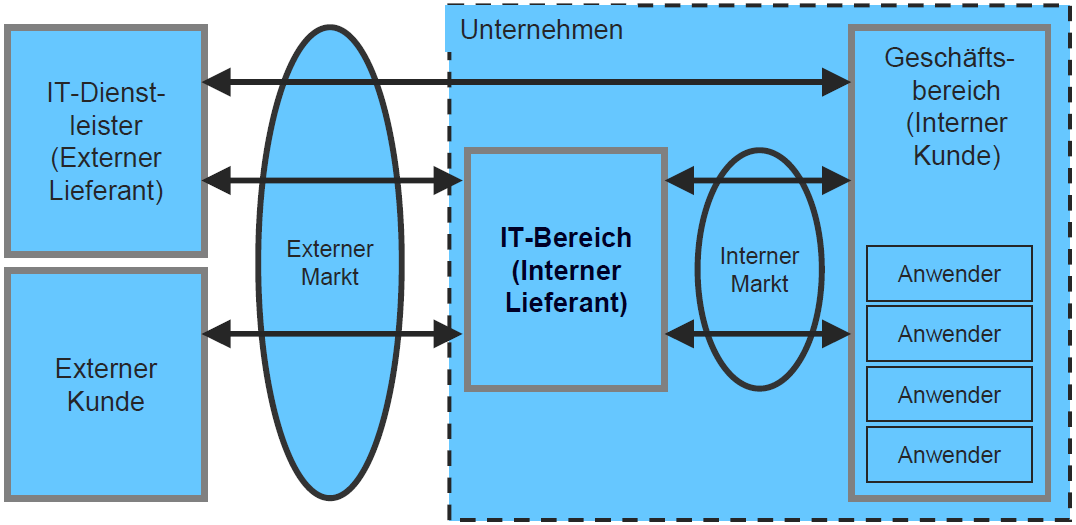
\includegraphics[width=0.9\textwidth]{einordnung_it_im_unternehmen}
    \\
    \cite[Quelle: Vgl.][]{FOM}
\end{figure}

IT Dienstleister kann an der IT vorbei direkt mit Geschäfztsbereich arbeiten, z.B. bei produktrelevanten Spezialanwendungen 
IT Bereich als Interner Lieferant: Equiptment, Zugänge, Lizenzen
Beziehung IT Abteilung <> Externe Kunden z.B. AWS -> erst für interne Zwecke gedacht, dann an Kunden verkauft

\begin{figure}[H]
    \caption{Organisationsformen der IT im Unternehmen}
    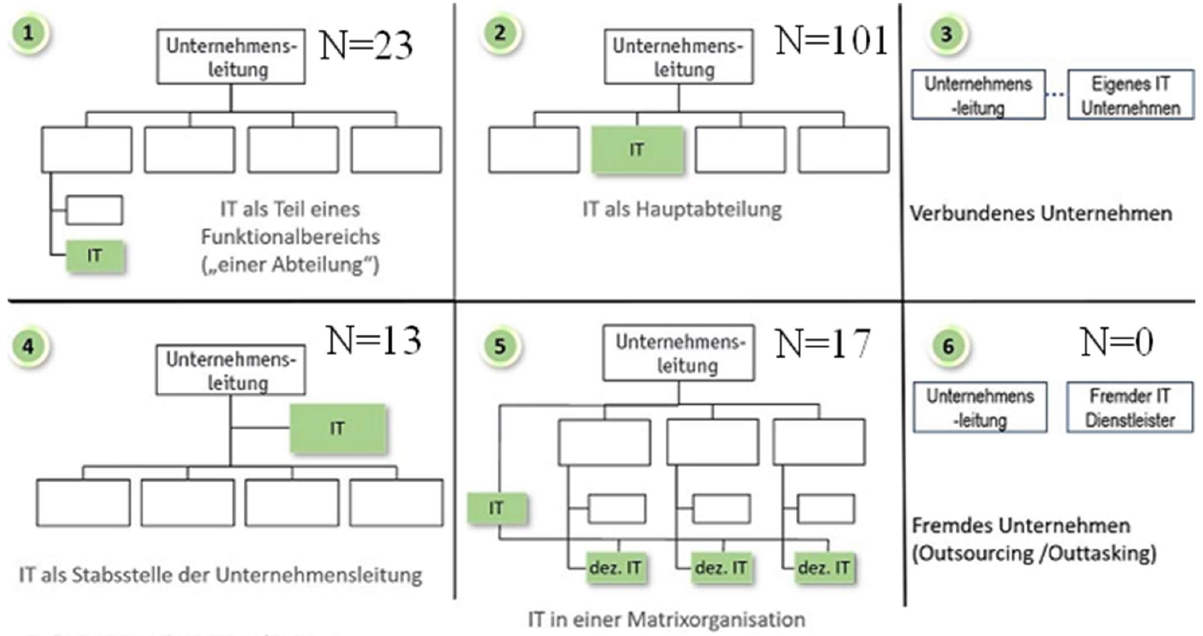
\includegraphics[width=0.9\textwidth]{organisationsformen}
    \\
    \cite[Quelle: Vgl.][]{FOM}
\end{figure}

\begin{itemize}
    \item Funktional: eher Mittelstand
    \item Hauptabteilung: Konzern IT Leiter hat Außenkontakt
    \item Stab: Nähe zur GL; keine Dursetzungskompetenz; sehr politisch; GL ist alleiniger Entscheider (auch bei neuen Technologien wie KI)
\end{itemize}

IT Bereich klassisch unterteilt in Entwicklung und Systembetrieb. 20\% - 30\% der Ressourcen fließen in die Systementwicklung, Rest in Systembetrieb. IT-Effektivität(X-Achse) zu IT-Komplexität (Y-Achse) ist exponentiell; Einsatz Produktionsfaktor IT (X-Achse) zu Nutzen ist logarithmisch. 
\\Daher: Wertbeitrag von IT-Investitionen auf der Grundlage klassischer IT-Architekturmodelle

IT ist "Enabler" für Organisation. IT und Geschäftsstrategie in Abhängigkeit. IT Wertschöpfung teils schwer definierbar. 

IT Wertbeitrag\\
\\IT wirkt indirekt über die Verbesserung der IT-Effektivität und IT-Effizienz auf das Geschäft
\begin{figure}[H]
    \caption{IT Wertbeitrag}
    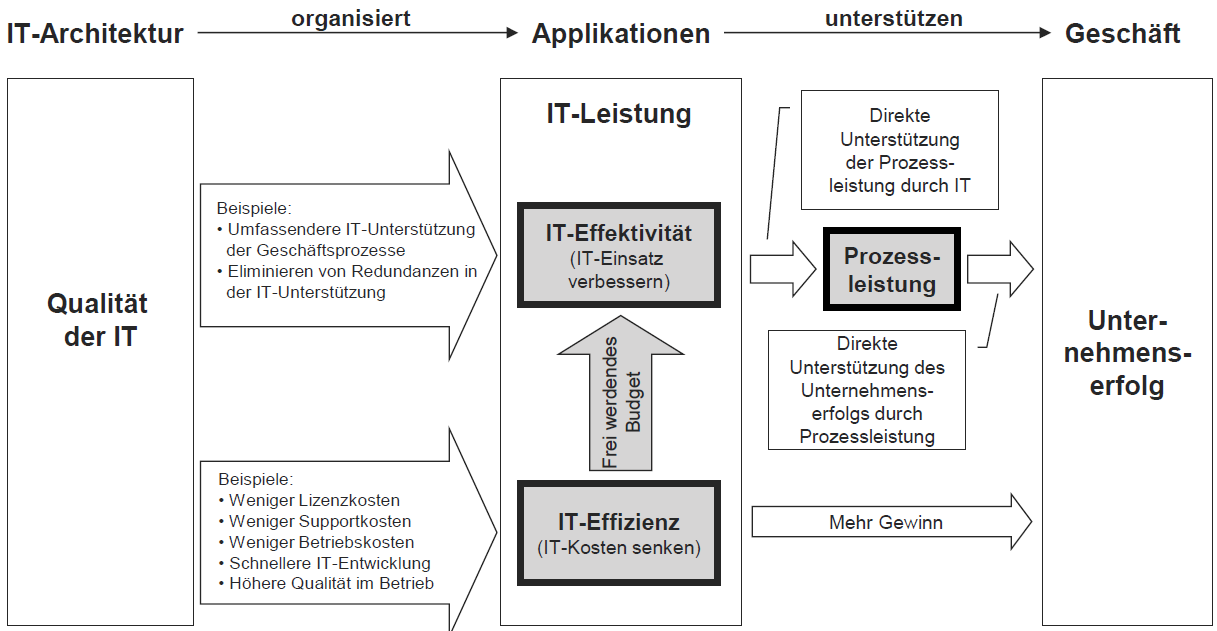
\includegraphics[width=0.9\textwidth]{it_wertbeitrag}
    \\
    \cite[Quelle: Vgl.][]{FOM}
\end{figure}
IT Effizienz: durch z.B. RPA, Code Assistant (schnellere Entwicklung), 
IT Effektivität: Integration ERP System, Weniger Clicks pro Prozess.

\begin{figure}[H]
    \caption{Gestaltungsdimensionen der IT}
    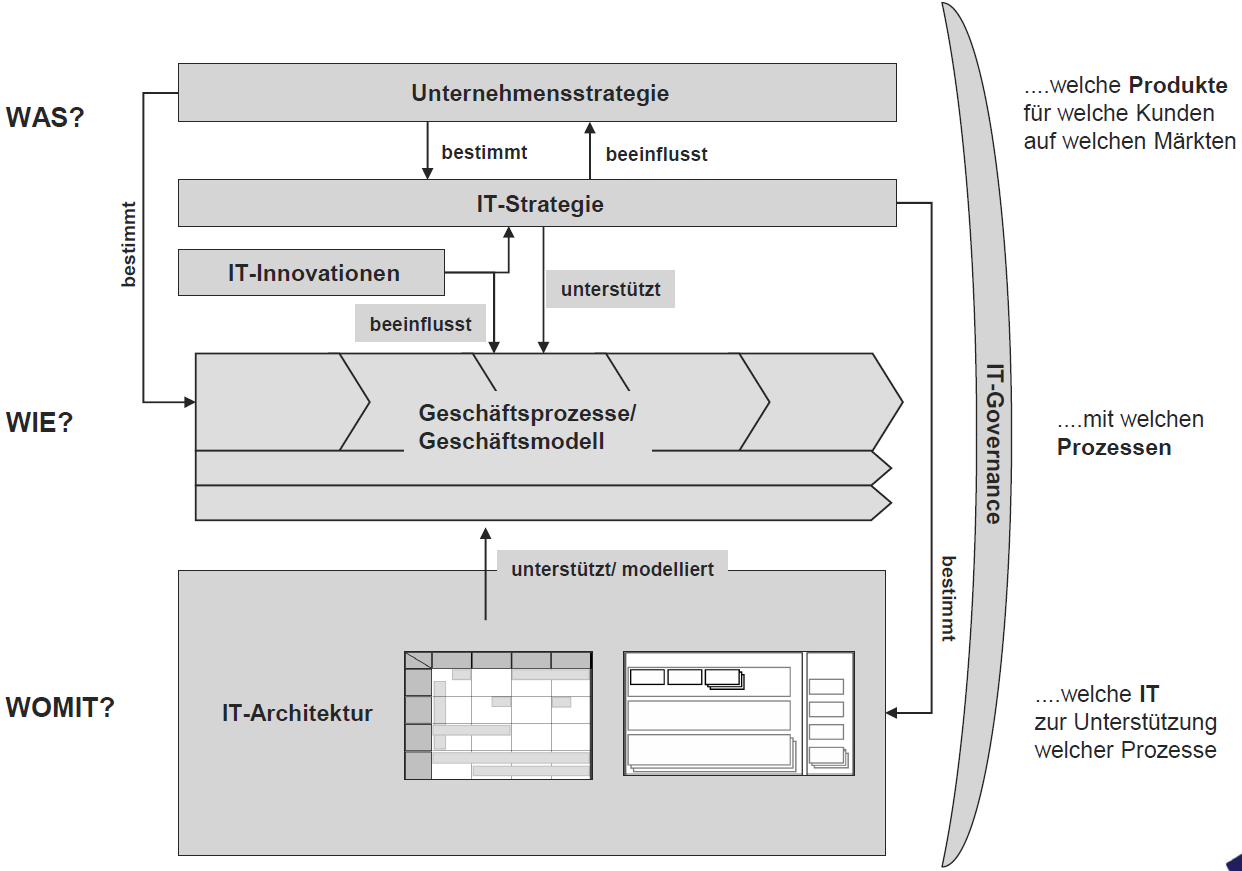
\includegraphics[width=0.9\textwidth]{gestaltungsdimensionen_IT}
    \\
    \cite[Quelle: Vgl.][]{FOM}
\end{figure}



\subsubsection{Vorüberlegungen}
Trichtermethode: Man beginnt mit der eigentlichen  Konklusion und überlegt dann, welche allgemeinen Teile dafür benötigt werden.

Welchen Mehrwert soll die Arbeit bieten \footnote{Diese Fu\ss note hat inhaltlich keinen Sinn. Es soll nur ein langer Text generiert werden, dass dieser Vermerk über zwei Zeilen reicht und bündig dargestellt wird.}? Auch darüber nachdenken, wie die Arbeit einen selbst weiter bringen kann. Studienverlauf prüfen. Welche Vorlesungen hat mich besonders interessiert? Wo liegen meine Stärken etc.

\begin{enumerate}
\item Themenfindung
\item Literaturrecherche
\item Gliederung/Motivationspapier erstellen
\item Betreuerauswahl (siehe Liste im \ac{OC})
\item Anmeldung (ab 141 Credits möglich)
\end{enumerate}

\subsubsection{Anregungen finden}
\begin{itemize}
\item \href{http://www.diplom.de}{www.diplom.de}
\item \href{http://www.hausarbeiten.de}{www.hausarbeiten.de}
\item Datenbanken aus Tools and Methods
\item etc.
\end{itemize}

\newpage
\subsection{Anfertigungsphase}
Die Anmeldung ist mittlerweile jeden Mittwoch möglich.
\begin{figure}[H]
\caption{FOM-Vorgaben zur Thesis im Online-Campus}
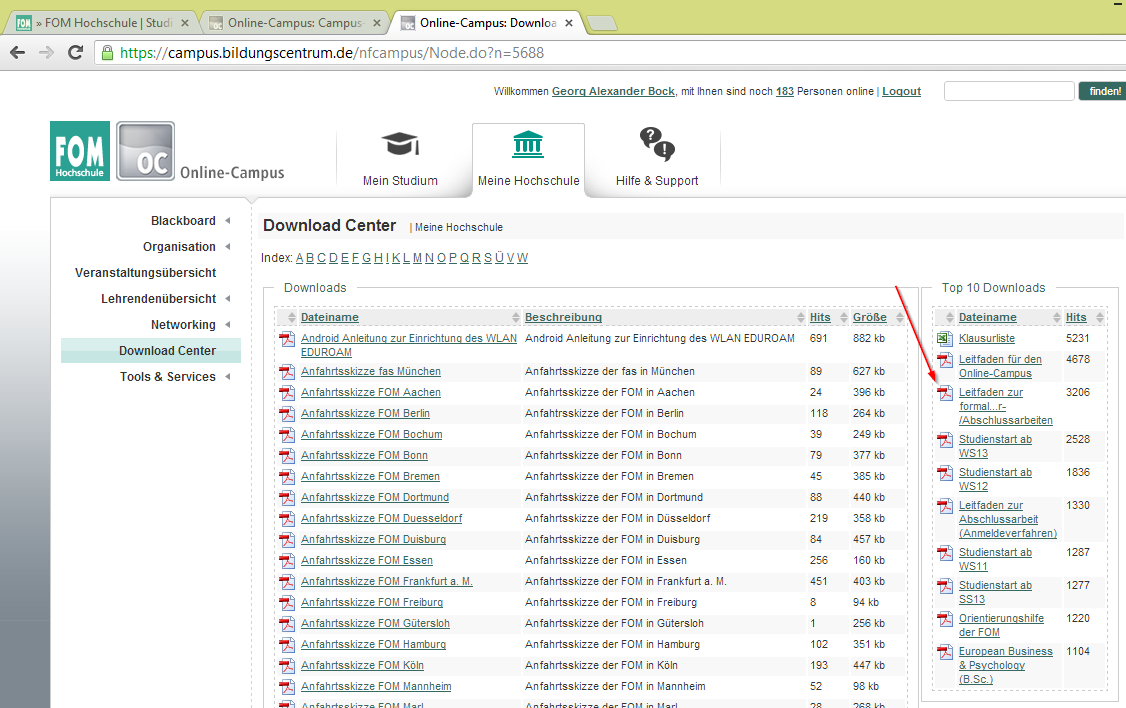
\includegraphics[width=0.9\textwidth]{campusDownload}
\\
\cite[Quelle: Vgl.][]{FOM}
\end{figure}

Laut Herrn Keller sollte der Umfang der Thesis (für eine gute Note) eher im Bereich der 60 Seiten liegen. Wie immer ist das vermutlich mit dem Betreuer abzustimmen. Die Liste der Dozenten, die Abschlussarbeiten betreuen, findet sich auch im \ac{OC}.

Zeit zur Erstellung der Thesis 2-4 Monate.

Es müssen zwei gedruckte Arbeiten abgegeben werden. Flüchtige Quellen als PDF ausgeben lassen und auf CD abgeben. Thesis zusätzlich digital einreichen. Beim Binden der Thesis auf Qualität achten. Haptik und erster Eindruck sind in der Bewertung \enquote{auch} wichtig. Arbeiten können in jedem FOM Studienzentrum abgegeben werden.

\subsection{Post-Abgabephase}
Nach Abgabe ca. 2 Wochen bis zum Kolloquium.

Kolloquium:
\begin{itemize}
\item Dauer: 30 Minuten
\item Präsentation (manche Prüfer wollen eine, andere nicht)
\item Betreuer vorher fragen was er möchte
\item Es gibt einen Frageteil, dieser bezieht sich auf die Arbeit, kann aber auch darüber hinaus gehen.
\item Der Tag des Kolloquiums steht auf der Endbenotung
\item Thesis und Kolloquium sind zwei getrennte Prüfungsbereiche. Für beide gibt es nur zwei Versuche.
\item Am Tag des Kolloquiums erhält man die Bestätigung, ob bestanden oder nicht
\end{itemize}
